\documentclass{sigchi}

% Use this command to override the default ACM copyright statement
% (e.g. for preprints).  Consult the conference website for the
% camera-ready copyright statement.

%% EXAMPLE BEGIN -- HOW TO OVERRIDE THE DEFAULT COPYRIGHT STRIP -- (July 22, 2013 - Paul Baumann)
%\toappear{One does not simply copy this document.}
%% EXAMPLE END -- HOW TO OVERRIDE THE DEFAULT COPYRIGHT STRIP -- (July 22, 2013 - Paul Baumann)

% Arabic page numbers for submission.  Remove this line to eliminate
% page numbers for the camera ready copy
% \pagenumbering{arabic}

% Load basic packages
\usepackage{balance}  % to better equalize the last page
\usepackage{graphics} % for EPS, load graphicx instead 
\usepackage[T1]{fontenc}
\usepackage{placeins}
\usepackage{txfonts}
\usepackage{mathptmx}
\usepackage[pdftex]{hyperref}
\usepackage{color}
\usepackage{booktabs}
\usepackage{textcomp}
\usepackage{pgfplots}
% Some optional stuff you might like/need.
\usepackage{microtype} % Improved Tracking and Kerning
% \usepackage[all]{hypcap}  % Fixes bug in hyperref caption linking
\usepackage{ccicons}  % Cite your images correctly!
\usepackage[utf8]{inputenc} % for a UTF8 editor only

% If you want to use todo notes, marginpars etc. during creation of your draft document, you
% have to enable the "chi_draft" option for the document class. To do this, change the very first
% line to: "\documentclass[chi_draft]{sigchi}". You can then place todo notes by using the "\todo{...}"
% command. Make sure to disable the draft option again before submitting your final document.
\usepackage{todonotes}

% Paper metadata (use plain text, for PDF inclusion and later
% re-using, if desired).  Use \emtpyauthor when submitting for review
% so you remain anonymous.
\def\plaintitle{Flash Crowd Online Student Enrollment System}
\def\plainauthor{Jan Keith Darunday, Ferriel Lisandro Melarpis, Toni-Jan Keith Monserrat, and Reginald Neil Recario}
\def\emptyauthor{}
\def\plainkeywords{Authors' choice; of terms; separated; by
  semicolons; include commas, within terms only; required.}
\def\plaingeneralterms{Documentation, Standardization}

% llt: Define a global style for URLs, rather that the default one
\makeatletter
\def\url@leostyle{%
  \@ifundefined{selectfont}{
    \def\UrlFont{\sf}
  }{
    \def\UrlFont{\small\bf\ttfamily}
  }}
\makeatother
\urlstyle{leo}

% To make various LaTeX processors do the right thing with page size.
\def\pprw{8.5in}
\def\pprh{11in}
\special{papersize=\pprw,\pprh}
\setlength{\paperwidth}{\pprw}
\setlength{\paperheight}{\pprh}
\setlength{\pdfpagewidth}{\pprw}
\setlength{\pdfpageheight}{\pprh}

% Make sure hyperref comes last of your loaded packages, to give it a
% fighting chance of not being over-written, since its job is to
% redefine many LaTeX commands.
\definecolor{linkColor}{RGB}{6,125,233}
\hypersetup{%
  pdftitle={\plaintitle},
% Use \plainauthor for final version.
%  pdfauthor={\plainauthor},
  pdfauthor={\emptyauthor},
  pdfkeywords={\plainkeywords},
  bookmarksnumbered,
  pdfstartview={FitH},
  colorlinks,
  citecolor=black,
  filecolor=black,
  linkcolor=black,
  urlcolor=linkColor,
  breaklinks=true,
}

% create a shortcut to typeset table headings
% \newcommand\tabhead[1]{\small\textbf{#1}}


% remove copyright
\makeatletter
\def\@copyrightspace{\relax}
\makeatother

% End of preamble. Here it comes the document.
\begin{document}

\title{\plaintitle}

%Jan Keith Darunday, Ferriel Lisandro Melarpis, Toni-Jan Keith Monserrat, and Reginald Neil Recario
\numberofauthors{4}
\author{%
  \alignauthor{Jan Keith Darunday\\
    \affaddr{Los Ba\~{n}os, Philippines}\\
    \email{jcdarunday@up.edu.ph}}\\
  \alignauthor{Ferriel Lisandro Melarpis\\
    \affaddr{Los Ba\~{n}os, Philippines}\\
    \email{fbmelarpis@up.edu.ph}}\\
  \alignauthor{Toni-Jan Keith Monserrat\\
    \affaddr{Los Ba\~{n}os, Philippines}\\
    \email{tonijanmonserrat@gmail.com}}\\
  \alignauthor{Reginald Neil Recario\\
    \affaddr{Los Ba\~{n}os, Philippines}\\
    \email{rcrecario@up.edu.ph}}\\
}

\maketitle

\begin{abstract}
One of the challenges of universities with high student populations in the Philippines is the implementation of
an online enrollment system. Many of these systems were not tested to handle sudden heavy influx of user connections
and the technologies used are not best-fitted for such events. In this research, we design and implement a system
that can perform well under sudden surges of users by applying the most recent technological advances and design techniques. 
We use Redis as the database for fast atomic database access, Rust as a language with Iron as the web server framework for faster 
serving of HTTP requests by removing the need for a garbage collector, and the split client-server architecture that allows
the offloading of heavy content to static servers. The implemented system was tested by running benchmarks on both the database and
the server that will handle HTTP requests and measuring the number of requests per second. From this, we can see how it will perform
during sudden heavy load that occur during the online registration period. The results proved the efficiency of the system by showing
that it can serve an average of 17,600 requests per second with the database serving 83,400 requests per second on a dual-core system.
Moreover, because the system is designed to be multithreaded and utilize all cores, the server should be able to linearly scale when
more cores are added making it able to serve more than 50,000 requests on a higher-end computer. In the future, improvements in the Iron
web server framework such as asynchronous IO, and faster parsing algorithms could further improve the server speed of the system
as they are some of the bottlenecks of the system.
\end{abstract}
% 
% \category{K.3.2}{Computing Milieux}{COMPUTERS AND EDUCATION }{Computer and Information Science Education }
% 
\keywords{student; information; registration; enrollment; Rust; Redis; static webapp}

\section{Introduction}

In academic institutions with large student populations such as campuses under
the University of the Philippines (UP) System, the implementation of an online registration
system for students is considered to be one of the biggest challenges as the system needs
to be capable of handling the surge of network connections from the whole student population
during the online registration period. Some of these systems were created by students studying 
in their respective universities and some of the others were created by software development
companies paid by the university. However, many of these systems failed
to address need of the institution that it serves due to issues like lack of budget, lack of development time,
use of wrong or outdated technologies, and lack of consultation of what the users actually need.

This research paper will use the enrollment system and online registration system in
the University of the Philippines as a context.

In the UP System, students are free to enlist into General Education (GE)
courses. These GE courses are courses that allow students from any degree program to enlist into
unlike major courses that are only available to certain degree programs. The
ability to choose one’s subjects implied that almost all students will need to
manually fill-up their list of courses to enroll to before the beginning of 
every semester. Moreover, courses are divided into sections each of which have 
a limited number of slots for students that it can accommodate. This meant that 
not only will the students need to manually check for conflicts in their 
schedules, they will also need to check if the course that they want to enlist 
in still has slots remaining.

The complexity of this process along with the increasing availability of Internet access to the public incited the development of computerized Online Registration Systems (ORS). These systems allowed the enlistment, cancellation, and swapping of slots for courses over the Internet. These systems also did the checking of conflicting subjects and availability of slots automatically so that students will not need to do them manually. In the University of the Philippines Los Baños (UPLB), the Online Registration System that is used as of the writing of this paper is called SystemOne. This system has undergone various revisions and improvements as old technology become deprecated by new ones and problems encountered in previous versions are fixed. The most recent one identifies itself as the third version and is code-named “Decaf”. However, this system did not prove to be efficient enough for the student population of UPLB despite several rewrites and revisions. This paper seeks to improve open this kind of online registration by fixing the problems encountered by SystemOne as a basis.

Because SystemOne is originally written in the PHP programming 
language which has been known to be slow, using a faster programming language 
would be an improvement. SystemOne also has its database connection as its 
bottleneck but it tries to solve this by using memcache as a caching system. 
However, this wasn't efficient enough as queries executed by the backend is too
dynamic which makes the results hard to cache. There are also lots of workarounds
that try to solve the race conditions that occur. Our system will try to solve this
by choosing a more feasible database system for sudden surges of requests.

\section{Related Work}

There is a limited number of papers that specifically discuss SystemOne. These papers mostly focus on the various modules that provide different kinds of functionality for SystemOne and the features to be created rather than the speed and feasibility of the use of the system. Suayan (1997) developed one of the first registration systems used in UPLB called the UPLB RegisNet \cite{suayan}. This system was designed to automate the pre-enlistment of subjects for students.

Meanwhile, the UPLB Academic Information System was created and had support for modularity. Through its modularity, various modules were created for it. Cruz (2001) created a Subjects module that gave it the ability to add, edit, and delete subjects from a list of subjects \cite{cruz} and Almodiel (2001) developed a module that allowed teachers to add, search, and view the grades of a student in their respective classes \cite{almodiel}. Enrique (2001) then developed a Schedule of Classes module that was responsible for managing and viewing the schedule of a subject, a room, or a teacher \cite{enrique}.

After a few years, Javier, et al. (2005) developed the first version of UPLB’s Online Registration System called SystemOne \cite{javier}. This system was also extensible through modularity. In this version, SystemOne used the Java programming language for implementing the Enlistor and Registrar module, PHP 5 for the Department module and MySQL as the Database Management System (DBMS).

In 2010, the development of the UPLB SystemOne V2 began. This version also used the Java programming language and the MySQL DBMS and was also modular. However, the difference of this new system from the previous system was that even the core functions were divided into modules and was developed separately.

In 2012, the third and current version of SystemOne was developed by the SystemOne Development Team. This system, unlike the previous versions that used Java, used the PHP programming language along with the MySQL DBMS. Like the second version, this system supports modules and its core functions are also implemented as modules.

There was one study that focused on the speed and response time of SystemOne. Crespo (2014) wrote a study entitled “Comparing the Response and Rendering Time of PHP-based against Javascript-based SystemOne” \cite{crespo}. This study did a comparison on how much faster or slower SystemOne would be had it been implemented in Javascript using the NodeJS interpreter. Her study detailed the performance of her own Javascript-based implementation against the PHP-based implementation. The results of her study showed that the Javascript-based implementation yielded a 52 percent increase in overall speed.

These results seem to be very promising considering the fact that NodeJS is known to not be able to take full advantage of a server computer that has multiple cores yet. This shows that SystemOne could have been faster if the right choices were made. These studies show a history of Online Registration Systems used in UPLB. It can be seen in the papers and articles cited that the use of the best and fastest technology has not really been given consideration.

\section{Methodology}

\subsection{Database}

As an information system, the speed of the system depends heavily on the speed of the database management system since most of the requests that it handles do modification of data. Because of this, Redis was chosen as it is a database management system that has low runtime overhead and very fast request-serving speeds with benchmarks showing hundreds of thousands of requests per second for atomic functions.

In order to achieve its speed, Redis sacrifices data integrity by writing and reading all data to and from the main memory of the system. This leads to possible data loss upon the occurance of a power interruption while Redis hasn't yet synchronized its data to permanent storage. However, this should not matter as long as the server has proper uninterruptible power supply systems in place. Even if such an event occurs, Redis uses sequential writing which will simply cancel out the latest writes causing a rollback rather than corrupting the whole database.

\subsection{Backend}

The backend is a server that serves a Representational State Transfer (REST) Application Programming Interface (API) through the Hypertext Transfer Protocol (HTTP). The implementation of the backend utilizes multithreading in order to be able to use all processor cores for the processing of HTTP requests. A thread will be spawned for every successful HTTP connection. This thread will handle its own associated connection and wait for a command before processing it and giving a reply. If a command is not received or completed after a specified amount of time, a timeout will occur and the connection will be dropped along with its corresponding thread being deallocated from the memory. 

\subsubsection{Conflict Checking}

Every time a modification or addition is done on the schedule of a student, the backend will check for conflicts before executing the specified action. In order to implement this, the students schedule is stored as a set of numbers that represent the index of each 15-minute block throughout the day beginning at 7:00 AM. For example, the number represents the time from 7:00AM to 7:15AM. This representation is also applied to the schedule of each subject. 

With the said representation of schedules, conflict checking is done by simply executing a set intersection of the schedule of the student and the schedule of the subject. If the resulting set does not have the size of zero, then it can be said that there is a conflict between the two schedules.

\subsubsection{Cross-Site HTTP Requests}

The system is designed to support HTTP Requests from specific domains
where the frontend code will be stored through the Access-Control-Allow-Origin header. 
This allows us to outsource the load added by frontend data being served as 
it will take a significant amount of networking bandwidth to serve the images and
scripts included. This will also allow the frontend to have heavier images and 
scripts without affecting the performance of the main server. 

\subsection{Frontend}

The frontend is a static web application that fires REST requests to the
backend server. Requests use HTTP methods such as GET, POST, PUT, and DELETE to 
specify how data on the server is specified. Some of the commands have the same URL
but is executed by specifying the HTTP method. For example, a PUT request on the schedule
URL enlists a subject while a DELETE request on the same URL will cancel a subject. the
server will then respond with the result in Javascript Object Notation (JSON) format that
includes the resulting data and the return code specifying the kind of error or if there is
no error.

A copy of the list of subjects and schedules in JSON format is also loaded with the backend
making subject searching fast and reducing API server load by not sending requests that are known 
to fail such as enlistment and waitlisting of already-conflicting subjects.

The static file server of the frontend can be served on a server with a caching service
like CloudFlare enabled which would cache the static web application into its own 
Content Delivery Network(CDN).

Moreover, the static web application can also be cached on the browser of the client by specifying Cache-Control headers. We can go even further by utilizing IndexDB, AppCache, and localStorage capabilities to store the frontend application which will completely store the application in the browser making it accessible even if the static server is down.

This setup also lessens the number of connections that the server will receive lessening the number of threads running in the backend. This also alleviates the additional load caused by students opening the site in multiple tabs and refreshing each tab repeatedly.

The design for the frontend tries to follow Material Design Specification by Google although not strictly. Along with this, it shall support mobile platforms by implementing Responsive Design. 

%TODO: Should be 1/2
\section{Evaluation}

The system is evaluated by its stability and efficiency.

The stability and efficiency of the system were evaluated by running benchmarks on the system. Information such as requests per second, time per request, and transfer rate of each function are collected. The system was also be tested if it can handle medium and heavy workloads by using load testing tools and services. These tests will use combinations of the different functions at ratios expected during actual use of the system. 

Benchmarks were ran on both the API server and the database management system. The API server is benchmarked by running the tools wrk and apachebench. These two tools apply load to the server by running thousands of connections and recording either the number of requests done after a certain duration or the time it takes for a specified number of requests to finish.

On the other hand, the database management system is benchmarked by running its own benchmarking tool that can benchmark server-side scripts and simulate its interaction with a specified number of keys which makes the evaluation of the speed of a script when there are a certain number of data on the server much easier.

\section{Results and Discussion}
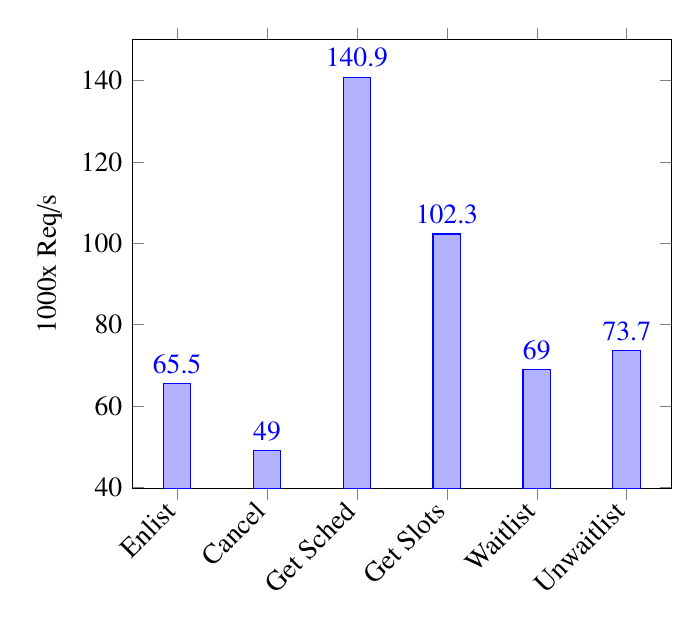
\begin{tikzpicture}
  \begin{axis}[ ybar, 
		legend style={at={(0.5,-0.2)}, 
		anchor=north,legend columns=-1}, 
		ylabel={1000x Req/s}, 
		symbolic x coords={Enlist, Cancel, Get Sched, Get Slots, Waitlist, Unwaitlist},
		xtick=data, 
		nodes near coords, 
		nodes near coords align={vertical}, 
		x tick label style={rotate=45,anchor=east}, ]
		\addplot coordinates {(Enlist,65.5) (Cancel,49.0) (Get Sched,140.9) (Get Slots,102.3) (Waitlist,69.0) (Unwaitlist,73.7)};
  \end{axis}
\end{tikzpicture}
\begin{center}
  Figure 1. Database requests per second on a Dual Core i7-5600U
\end{center}
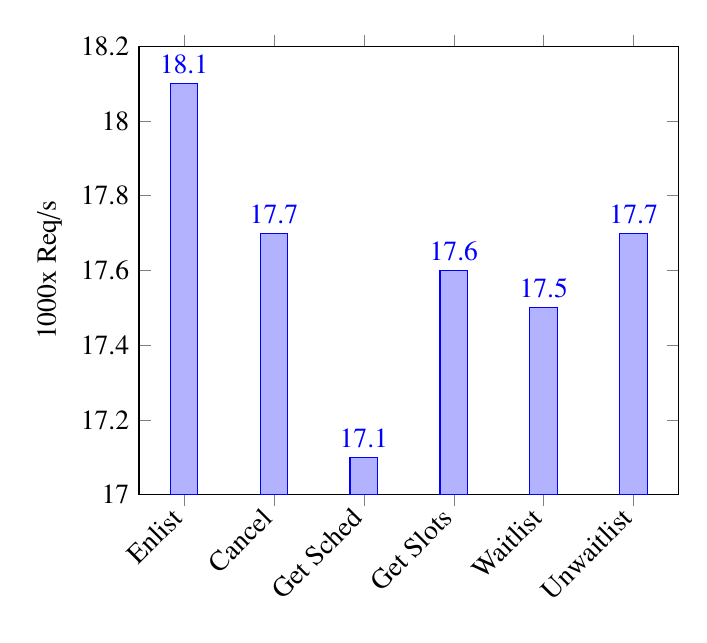
\begin{tikzpicture}
  \begin{axis}[ ybar, 
		legend style={at={(0.5,-0.2)}, 
		anchor=north,legend columns=-1}, 
		ylabel={1000x Req/s}, 
		symbolic x coords={Enlist, Cancel, Get Sched, Get Slots, Waitlist, Unwaitlist},
		xtick=data, 
		nodes near coords, 
		nodes near coords align={vertical}, 
		x tick label style={rotate=45,anchor=east}, ]
		\addplot coordinates {(Enlist,18.1) (Cancel,17.7) (Get Sched,17.1) (Get Slots,17.6) (Waitlist,17.5) (Unwaitlist,17.7)};
  \end{axis}
\end{tikzpicture}
\begin{center}
  Figure 2. API server requests per second on a Dual Core i7-5600U
\end{center}

In Figure 1, it is shown that the database management system, Redis, was able to serve an average of 83,400 requests per second on an Intel Core i7-5600U. It should be noted that Redis is only able to utilize a single core so scaling through sharding will linearly increase this serving speed.

It is also noted that the command for retrieving the schedule is processed the fastest at 140,900 requests per second. This is because it is the least complex command that consists only of a single read request to the database after input validation. On the other hand, it can be seen that the command for cancellation of subjects is processed the slowest. This is due to it being the most complex command involving input validation, retrieval and verification of enlisted subject, actuall removal of enlisted subject, retrieval of the front element in the waitlist queue, conflict checking of subject against the schedule of the waitlister, and, finally, the enlistment of the waitlister.

In Figure 2, it can be seen that the requests per second went down from the database average of 83,400 to 17,600 with low deviation on the same machine. This shows that the overhead caused by the API server is the bottleneck in this setup. Early tests in the API server showed higher number of requests per second that can be blamed on the addition of URL parsers, data persistence middlewares, and JSON encoders that likely caused the reduction in the serving-speed. However, these benchmarks only shows its performance on a dual core system and the API server is highly multithreaded which implies that it could perform much faster on multicore and multiprocessor servers. Moreover, the API server can also be scaled by using a load balancer with it running on multiple servers that share the same database. 

\section{Summary and Conclusion}

Based on the results of the system evaluation, we can conclude that the system is efficient enough to handle most universities with large student populations such as the University of the Philippines Los Baños that has around 13,710 students even if each student does an API requests once per second. It can be implied that it can also serve populations much larger than the benchmark results through scaling. 
% REFERENCES FORMAT
% References must be the same font size as other body text.
\bibliographystyle{sigchi}
\bibliography{sp2-paper}

%\cleardoublepage

\end{document}

%%% Local Variables:
%%% mode: latex
%%% TeX-master: t
%%% End:
